% The format is taken (and subsequently updated to work with new package updates) from: https://github.com/kenfehling/latex-cheatsheet
\documentclass[10pt,landscape,letterpaper]{article}
\usepackage[utf8]{inputenc}
\usepackage[USenglish]{babel}
\usepackage[T1]{fontenc}
\usepackage{lipsum}
\usepackage[explicit]{titlesec}
%\usepackage[LY1,T1]{fontenc}
%\usepackage{frutigernext}
%\usepackage[lf,minionint]{MinionPro}
\usepackage{tikz}
\usetikzlibrary{shapes,positioning,arrows,fit,calc,graphs,graphs.standard}
\usepackage[nosf]{kpfonts}
\usepackage[t1]{sourcesanspro}
\usepackage{multicol}
\usepackage{wrapfig}
\usepackage[top=0mm,bottom=1mm,left=0mm,right=1mm]{geometry}
\usepackage[framemethod=tikz]{mdframed}
\usepackage{microtype}
\usepackage{pdfpages}
\usepackage{listings}
\usepackage{xcolor}
\usepackage{mathtools}
\usepackage{enumitem}
\usepackage{booktabs}
\usepackage{tabularx}
\usepackage[super]{nth}

\renewcommand\tabularxcolumn[1]{m{#1}}
\renewcommand\arraystretch{1.25}

\let\bar\overline

\definecolor{myblue}{cmyk}{1,.72,0,.38}

\def\firstcircle{(0,0) circle (1.5cm)}
\def\secondcircle{(0:2cm) circle (1.5cm)}

\colorlet{circle edge}{myblue}
\colorlet{circle area}{myblue!5}

\definecolor{mypurple}{rgb}{0.4,0.16,0.46}

\tikzset{>=stealth,filled/.style={fill=circle area, draw=circle edge, thick},
    outline/.style={draw=circle edge, thick}}
    
\pgfdeclarelayer{background}
\pgfsetlayers{background,main}

\everymath\expandafter{\the\everymath \color{myblue}}
\everydisplay\expandafter{\the\everydisplay \color{myblue}}

\renewcommand{\baselinestretch}{.8}
\pagestyle{empty}

\newcommand\bold[1]{{\bfseries #1}}

\global\mdfdefinestyle{header}{%
linecolor=gray,linewidth=1pt,%
leftmargin=0mm,rightmargin=0mm,skipbelow=0mm,skipabove=0mm,
}

\newcommand{\header}{
\begin{mdframed}[style=header]
\footnotesize
\sffamily
CS2 Final Reference Sheet\\
~Page~\thepage~of~8
\end{mdframed}
}

%%% Code Styles

\definecolor{codegreen}{rgb}{0,0.6,0}
\definecolor{codegray}{rgb}{0.5,0.5,0.5}
\definecolor{codepurple}{rgb}{0.58,0,0.82}

\lstdefinestyle{mystyle}{
    commentstyle=\color{codegray},
    keywordstyle=\color{magenta},
    numberstyle=\tiny\color{codepurple},
    stringstyle=\color{codegreen},
    basicstyle=\ttfamily\footnotesize,
    breakatwhitespace=false,         
    breaklines=true,                 
    captionpos=b,                    
    keepspaces=true,                 
    numbers=none,                    
    numbersep=5pt,                  
    showspaces=false,                
    showstringspaces=false,
    showtabs=false,                  
    tabsize=2
}

\lstset{style=mystyle}

%%%

\makeatletter % Author: https://tex.stackexchange.com/questions/218587/how-to-set-one-header-for-each-page-using-multicols
\renewcommand{\section}{\@startsection{section}{1}{0mm}%
                                {.2ex}%
                                {.2ex}%x
                                {\color{myblue}\sffamily\small\bfseries}}
\renewcommand{\subsection}{\@startsection{subsection}{1}{0mm}%
                                {.2ex}%
                                {.2ex}%x
                                {\sffamily\bfseries}}
%\renewcommand{\subsubsection}{\@startsection{subsubsection}{1}{0mm}%
                                %{.2ex}%
                                %{.2ex}%x
                                %{\sffamily\small}}

\def\multi@column@out{%
   \ifnum\outputpenalty <-\@M
    \speci@ls \else
    \ifvoid\colbreak@box\else
      \mult@info\@ne{Re-adding forced
                break(s) for splitting}%
      \setbox\@cclv\vbox{%
       \unvbox\colbreak@box
       \penalty-\@Mv
       \unvbox\@cclv}%
    \fi
   \splittopskip\topskip
   \splitmaxdepth\@maxdepth
   \boxmaxdepth\@maxdepth
   \dimen@\@colroom
   \divide\skip\footins\col@number
   \ifvoid\footins \else
      \leave@mult@footins
   \fi
   \ifvbox \@kludgeins
     \advance \dimen@ -\ht\@kludgeins
     \ifdim \wd\@kludgeins>\z@
        \shr@nkingtrue
     \fi
   \fi
   \process@cols\mult@firstbox{%
        %%%%% START CHANGE
        \ifnum\count@=\numexpr\mult@rightbox+2\relax
                  \setbox\count@\vsplit\@cclv to \dimexpr \dimen@-1cm\relax
        \setbox\count@\vbox to \dimen@{\vbox to 1cm{\header}\unvbox\count@\vss}%
        \else
              \setbox\count@\vsplit\@cclv to \dimen@
        \fi
        %\setbox\count@
            %\vsplit\@cclv to\dimen@
        %%%%% END CHANGE
            \set@keptmarks
            \setbox\count@
                 \vbox to\dimen@
                  {\unvbox\count@
                   \ifshr@nking
                    \vfilmaxdepth\fi}%
           }%
   \setbox\mult@rightbox
       \vsplit\@cclv to\dimen@
   \set@keptmarks
   \setbox\mult@rightbox\vbox to\dimen@
          {\unvbox\mult@rightbox
           \ifshr@nking\vfilmaxdepth\fi}%
   \ifvoid\@cclv \else
       \unvbox\@cclv
       \ifnum\outputpenalty=\@M
       \else
          \penalty\outputpenalty
       \fi
       \ifvoid\footins\else
         \PackageWarning{multicol}%
          {I moved some lines to
           the next page.\MessageBreak
           Footnotes on page
           \thepage\space might be wrong}%
       \fi
       \ifnum \c@tracingmulticols>\thr@@
                    \hrule\allowbreak \fi
   \fi
   \ifx\@empty\kept@firstmark
      \let\firstmark\kept@topmark
      \let\botmark\kept@topmark
   \else
      \let\firstmark\kept@firstmark
      \let\botmark\kept@botmark
   \fi
   \let\topmark\kept@topmark
   \mult@info\tw@
        {Use kept top mark:\MessageBreak
          \meaning\kept@topmark
         \MessageBreak
         Use kept first mark:\MessageBreak
          \meaning\kept@firstmark
        \MessageBreak
         Use kept bot mark:\MessageBreak
          \meaning\kept@botmark
        \MessageBreak
         Produce first mark:\MessageBreak
          \meaning\firstmark
        \MessageBreak
        Produce bot mark:\MessageBreak
          \meaning\botmark
         \@gobbletwo}%
   \boxmaxdepth\maxdimen
   \setbox\@cclv\vbox{\unvbox\partial@page
                      \page@sofar}%
   \@makecol\@outputpage
     \global\let\kept@topmark\botmark
     \global\let\kept@firstmark\@empty
     \global\let\kept@botmark\@empty
     \mult@info\tw@
        {(Re)Init top mark:\MessageBreak
         \meaning\kept@topmark
         \@gobbletwo}%
   \global\@colroom\@colht
   \global \@mparbottom \z@
   \global \@textfloatsheight \z@
   \process@deferreds
   \@whilesw\if@fcolmade\fi{\@outputpage
      \global\@colroom\@colht
      \process@deferreds}%
   \mult@info\@ne
     {Colroom:\MessageBreak
      \the\@colht\space
              after float space removed
              = \the\@colroom \@gobble}%
    \set@mult@vsize \global
  \fi}

  % aligned substack 'subalign'
  % alignment point is set via & (uses preceeding char)
  % stolen from: https://tex.stackexchange.com/questions/198771/align-in-substack#answer-198806
  \newcommand{\subalign}[1]{%
      \vcenter{%
          \Let@ \restore@math@cr \default@tag
          \baselineskip\fontdimen10 \scriptfont\tw@
          \advance\baselineskip\fontdimen12 \scriptfont\tw@
          \lineskip\thr@@\fontdimen8 \scriptfont\thr@@
          \lineskiplimit\lineskip
          \ialign{\hfil$\m@th\scriptstyle##$&$\m@th\scriptstyle{}##$\hfil\crcr
              #1\crcr
          }%
      }%
  }

\makeatother
\setlength{\parindent}{0pt}

\titleformat{\subsubsection}{\sffamily\bfseries\small\color{mypurple}}{\thesubsubsection}{0mm}{#1:}{}

\titlespacing{\subsubsection}{0pt}{.2ex}{.2ex}


\setlist{leftmargin=*,labelindent=\parindent}

\newcommand\arraytable[8]{
    \begin{tabularx}{\linewidth}{|X|X|X|X|X|X|X|X|}
        \hline
        #1 & #2 & #3 & #4 & #5 & #6 & #7 & #8 \\
        \hline
    \end{tabularx}
    \begin{tabularx}{\linewidth}{XXXXXXXX}
        1 & 2 & 3 & 4 & 5 & 6 & 7 & 8\\
    \end{tabularx}
}

\begin{document}
\footnotesize
%\small
\begin{multicols*}{5}
    \section{Java}
\subsection*{ArrayList}
A resizable array.
\subsection*{LinkedList}
A list of elements where ea.\ element points to the next.
\subsection*{ArrayDeque}
A resizable array that acts like a double ended queue, which means that you can enqueue
and dequeue elements from both ends of the queue. This can be used as either a stack or a normal queue.
\subsection*{TreeSet}
An ordered set of unique values.
\subsection*{TreeMap}
Ordered keys mapped to values.
\subsection*{HashSet}
Unordered keys mapped to values.
\subsection*{HashMap}
An unordered set of unique values.
\subsection*{Priority Queue}
min or max, not both.
\begin{lstlisting}[language=Java,basicstyle=\tiny]
// Enqueue/Dequeue: O(log(n))
pQueue.remove();
pQueue.add();
pQueue.poll();

// Retrieval: O(1)
pQueue.peek();
pQueue.element();
pQueue.size();
\end{lstlisting}
\subsection*{Custom Sorting}
\begin{lstlisting}[language=Java,basicstyle=\tiny]
import java.util.Arrays;
import java.util.Comparator;

Arrays.sort(ToSort,
    new Comparator<ToSortClass>() {
        @Override
        public int compare(
            ToSortClass o1, ToSortClass o2
        ) {
            return Integer.compare(o1.value,
                                   o2.value);
        }
    }
);
\end{lstlisting}


    \section{Backtracking}
Recursion, try ea.\ possibility and go next, if no work go back
\begin{lstlisting}[language=Java,basicstyle=\tiny]
// ex: Sudoku
for (int i=1;i<=9;i++) { // place 1-9 for sudoku
  if (check(r,c,i)) { // if can place value i
    grid[r][c]=i; // place it
    if (solve(r,c+1)) { // solve w/ board next pos
      return true; // it's solved
    }
    // backtrack, rm val for later calls
    grid[r][c]=0;
  }
}
\end{lstlisting}

    \section{Data Structures}
\subsection*{Disjoint Sets}
A set of sets. Each set has a marked "leader" element.
{\footnotesize Two sets $A$ and $B$ are \textbf{disjoint} if $A\cap B=\emptyset$}

\subsubsection*{Array Representation}
Value in any given index corresponds to its direct parent.
Value will be the same as the index if it is the "root" of a tree set or is just an individual value.

Find: Returns the marked "leader" element of a set.

\subsubsection*{Union Operator}
(prioritize smaller tree height)

Merges two disjoint sets together.
If visualizing as a tree set,
take the tree with the smaller height,
and merge it into the taller tree.

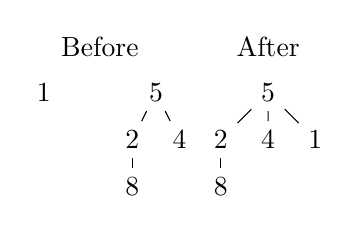
\begin{tikzpicture}[scale=0.4]
    \node (1) at (0,0) {1};
    \node (5) [right=of 1] {$5$}
        child {node (2) {2}
            child {node (8) {8}}
        }
        child {node (4) {4}};
    \node (5a) [right=of 5] {5}
        child {node (2a) {2}
            child {node (8a) {8}}
        }
        child {node (4a) {4}}
        child {node (1a) {1}};
    \node (before) [above=1mm of $(1.north)!0.5!(5.north)$] {Before};
    \node (after) [above=1mm of 5a] {After};
\end{tikzpicture}

\subsubsection*{Path Compression}
(findset on 8)

\begin{tikzpicture}[scale=0.35]
    \node (5) [right=of 1] {$1$}
        child{node (1) {5}
            child {node (2) {2}
                child {node (8) {8}}
            }
            child {node (4) {4}}
        };
    \node (5a) [right=of 5] {1}
        child {node (4a) {2}}
        child {node (1a) {8}}
        child {node (2a) {5}
            child {node (8a) {4}}
        };
    \node (before) [above=1mm of 5] {Before};
    \node (after) [above=1mm of 5a] {After};
\end{tikzpicture}

\arraytable{1}{5}{7}{5}{1}{7}{7}{2}

First, you find the root of this tree which is 1.
Then you go through the path again, starting at 8,
changing the parent of each of the nodes on that path to 1.

\arraytable{1}{5}{7}{5}{1}{7}{7}{1}

Then, you take the 2 that was previously stored in index 8,
and then change the value in that index to 1.

\subsection*{2-4 Trees}

num of children is equal to entries + 1 || 0

\subsubsection*{Insertion}
\resizebox{\linewidth}{!}{%
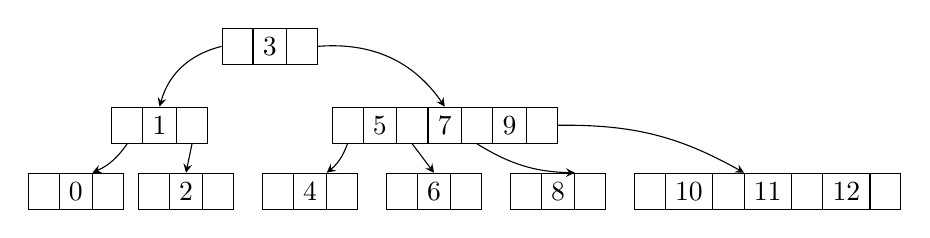
\begin{tikzpicture}[
    scale=0.1,
    NBox/.style={
        rectangle split,
        rectangle split horizontal,
        draw
    },
    T/.style={
        rectangle split parts=3
    }
    ]
    \node[NBox,T] (root) at (4,0) {\nodepart{two} 3};
    \node[NBox,T] (leftch) [below left=15pt and 5pt of root] {\nodepart{two} 1};
    \node[NBox,T] (leftchrch) [below=15pt and 5pt of leftch.three] {\nodepart{two} 2};
    \node[NBox,T] (leftchlch) [left=15pt and 5pt of leftchrch] {\nodepart{two} 0};
    \node[NBox,rectangle split parts=7] (rightch) [below right=15pt and 5pt of root] {\nodepart{two} 5 \nodepart{four} 7 \nodepart{six} 9};
    \node[NBox,T] (rightchlch) [right=10pt of leftchrch] {\nodepart{two} 4};
    \node[NBox,T] (rightchmch) [right=10pt of rightchlch] {\nodepart{two} 6};
    \node[NBox,T] (rightchrch) [right=10pt of rightchmch] {\nodepart{two} 8};
    \node[NBox,rectangle split parts=7] (rightchchr) [right=10pt of rightchrch] {\nodepart{two} 10 \nodepart{four} 11 \nodepart{six} 12};
    
    \path[->]
    (root.one west) edge [bend right=30] (leftch.two north)
    (leftch.three south) edge (leftchrch.two north)
    (leftch.one south) edge [bend left=15] (leftchlch.two split north)
    (root.three east) edge [bend left=30] (rightch.four north)
    (rightch.one south) edge [bend left=15] (rightchlch.two split north)
    (rightch.three south) edge (rightchmch.two north)
    (rightch.five south) edge [bend right=15] (rightchrch.two split north)
    (rightch.seven east) edge [bend left=15] (rightchchr.three split north);
\end{tikzpicture}
}

{\tiny Insert 13: 4 node. Split it. Push 11 up to parent. Parent is a 4 node, push 7 up.}

\resizebox{\linewidth}{!}{%
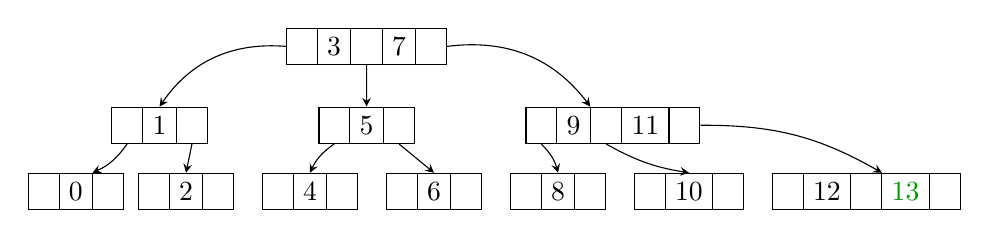
\begin{tikzpicture}[
    scale=0.1,
    NBox/.style={
        rectangle split,
        rectangle split horizontal,
        draw
    },
    T/.style={
        rectangle split parts=3
    }
    ]
    \node[NBox,rectangle split parts=5] (root) at (8,0) {\nodepart{two} 3 \nodepart{four} 7};
    \node[NBox,T] (midch) [below=15pt of root] {\nodepart{two} 5};
    \node[NBox,T] (leftch) [left=40pt of midch] {\nodepart{two} 1};
    \node[NBox,T] (leftchrch) [below=15pt and 5pt of leftch.three] {\nodepart{two} 2};
    \node[NBox,T] (leftchlch) [left=15pt and 5pt of leftchrch] {\nodepart{two} 0};
    \node[NBox,rectangle split parts=5] (rightch) [right=40pt of midch] {\nodepart{two} 9 \nodepart{four} 11};
    \node[NBox,T] (rightchlch) [right=10pt of leftchrch] {\nodepart{two} 4};
    \node[NBox,T] (rightchmch) [right=10pt of rightchlch] {\nodepart{two} 6};
    \node[NBox,T] (rightchrch) [right=10pt of rightchmch] {\nodepart{two} 8};
    \node[NBox,T] (rightchchrl) [right=10pt of rightchrch] {\nodepart{two} 10};
    \node[NBox,rectangle split parts=5] (rightchchr) [right=10pt of rightchchrl] {\nodepart{two} 12 \nodepart{four} \color{codegreen}13};
    
    \path[->]
    (root.one west) edge [bend right=30] (leftch.two north)
    (leftch.three south) edge (leftchrch.two north)
    (leftch.one south) edge [bend left=15] (leftchlch.two split north)
    (root.five east) edge [bend left=30] (rightch.two split north)
    (root.three south) edge (midch.two north)
    (midch.one south) edge [bend right=15] (rightchlch.two north)
    (midch.three south) edge (rightchmch.two north)
    (rightch.one south) edge [bend left=15] (rightchrch.two north)
    (rightch.three south) edge [bend right=10] (rightchchrl.two north)
    (rightch.five east) edge [bend left=15] (rightchchr.three split north);
\end{tikzpicture}
}

{\tiny can push up 2nd or 3rd value (3rd is more common)}

\subsubsection*{Deletion}

\begin{enumerate}
    \item Find key to remove and replace w/ next higher key.
    \item If sibling > 1 key, steal an adjacent key, make taht the parent and bring down the current parent.
    \item If no adjacent sibling has greater than one key, steal a key from a parent.
    \item If parent is the root and contains only one key and sibling has only one key, fuse it into a key node and make it the new root.
\end{enumerate}

Delete 20 from the following 2-4 tree.

\resizebox{\linewidth}{!}{%
    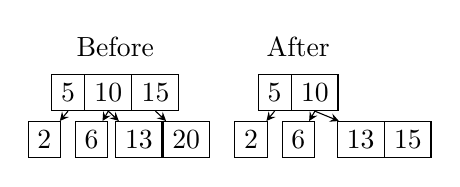
\begin{tikzpicture}[
        scale=0.4,
        Node/.style ={
            rectangle split,
            rectangle split horizontal,
            rectangle split parts=#1,
            draw,
        },
        Node/.default=3,
        edge from parent/.style ={draw,-stealth}
    ]
    \node[Node=3] (broot) at (4,0) {
            \nodepart{one} 5
            \nodepart{two} 10
            \nodepart{three} 15
        }
        child {node[Node=1] (b2) {2}
            [parent anchor=one south]
        }
        child {node[Node=1] (b6) {6}
            [parent anchor=two south]
        }
        child {node[Node=1] (b13) {13}
            [parent anchor=two south]
        }
        child {node[Node=1] (b20) {20}
            [parent anchor=three south]
        };

    \node[Node=2] (aroot) [right=of broot] {
            \nodepart{one} 5
            \nodepart{two} 10
        }
        child {node[Node=1] (a2) {2}
            [parent anchor=one south]
        }
        child {node[Node=1] (a6) {6}
            [parent anchor=two south]
        }
        child {node[Node=2] (a13) [right=0.8em of a6] {
                \nodepart{one} 13
                \nodepart{two} 15
            }
            [parent anchor=two south]
        };

    \node (before) [above=1mm of broot] {Before};
    \node (after) [above=1mm of aroot] {After};

    \end{tikzpicture}
}
\subsection*{Binary Tree Relationships}
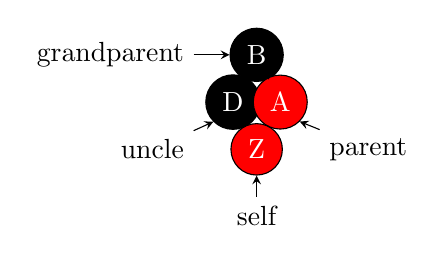
\begin{tikzpicture}[
    scale=0.4,
    blk/.style ={
        circle,
        white,
        fill=black,
        draw=black
    },
    rd/.style ={
        circle,
        white,
        fill=red,
        draw=black
    }
    ]
    \node[blk] (grandparent) at (0,0) {B}
        child{node[blk] (uncle) {D}}
        child{node[rd] (parent) {A}
              child{node[rd] (self) {Z}}
              child[missing]};

    \path[->] +(-2,0) node[left] {grandparent} edge (grandparent.west);
    \path[->] +(-2,-3) node[left] {uncle} edge (uncle.south west);
    \path[->] +(2,-3) node[right] {parent} edge (parent.south east);
    \path[->] +(0,-4.5) node[below] {self} edge (self.south);
\end{tikzpicture}

\subsection*{Red-Black Trees}
\begin{enumerate}
    \item A node is either {\color{red}red} or black.
    \item The root and leaves (NIL) are black.
    \item If a node is {\color{red}red}, then its children are black.
    \item All paths from a node to its NIL descendants contain the same number of black nodes.
    \item The longest path (root to farthest NIL) is no more than twice the length of the shortest path (root to nearest NIL).
        \scriptsize{
        \begin{itemize}
            \item Shortest path: all black nodes
            \item Longest path: alternating {\color{red}red} and black
        \end{itemize}}
\end{enumerate}

\subsubsection*{Insertion}
Strategy:
\begin{enumerate}
    \item Insert Z and color it {\color{red}red}
    \item Recolor and rotate nodes to fix violation
\end{enumerate}
{\bfseries Z is illegal scenarios}
\begin{enumerate}%
    \item[0.] Z = root $\to$ color black
    \item[1.] Z.uncle = {\color{red}red} $\to$ recolor
    \item[2.] {\scriptsize Z.uncle = {\bfseries black}(triangle) $\to$ rotate Z.parent}\\
        \resizebox{!}{5em}{% Black triangle diagram
        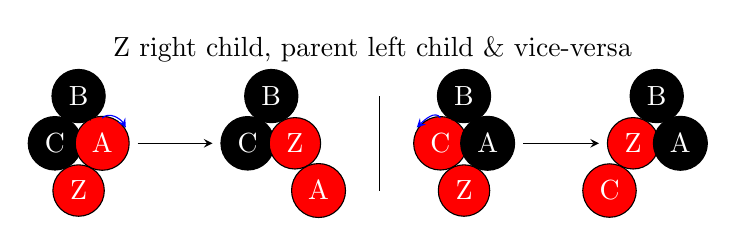
\begin{tikzpicture}[
            scale=0.4,
            blk/.style ={
                circle,
                white,
                fill=black,
                draw=black
            },
            rd/.style ={
                circle,
                white,
                fill=red,
                draw=black
            }
            ]
            \node[blk] (grandparent) at (0,0) {B}
                child{node[blk] (uncle) {C}}
                child{node[rd] (parent) {A}
                    child{node[rd] (self) {Z}}
                    child[missing]};

            \path[->,blue] ($(parent)+(0,0.8)$) edge [in=120,out=45] ($(parent)+(0.75,0.5)$);

            \node () [above right=1mm of grandparent] {Z right child, parent left child \& vice-versa};

            \node[blk] (agrandparent) [right=5em of grandparent] {B}
                child{node[blk] (auncle) {C}}
                child{node[rd] (aparent) {Z}
                    child[missing]
                    child{node[rd] (aself) {A}}};

            \path[->] (parent.east) ++(0.25,0) edge ($(auncle.west)+(-0.25,0)$);

            %% Mirrored

            \node[blk] (mgrandparent) [right=5em of agrandparent] {B}
                child{node[rd] (muncle) {C}
                    child[missing]
                    child{node[rd] (mself) {Z}}
                }
                child{node[blk] (mparent) {A}};

            \path[->,blue] ($(muncle)+(0,0.8)$) edge [in=45,out=120] ($(muncle)+(-0.75,0.5)$);

            \node[blk] (magrandparent) [right=5em of mgrandparent] {B}
                child{node[rd] (mauncle) {Z}
                    child{node[rd] (maself) {C}}
                    child[missing]
                }
                child{node[blk] (maparent) {A}};

            \path[->] (mparent.east) ++(0.25,0) edge ($(mauncle.west)+(-0.25,0)$);

            %% Anti-confusion mirror line
            \draw[draw] let \p1 = ($(aself)!0.5!(muncle)$),
                \p2 = (maself) in ($(\x1,0)$) -- +(0,\y2);
            %% Above line is overly complicated for what it is

        \end{tikzpicture}
        }
    \item[3.] {\scriptsize Z.uncle = {\bfseries black}(line) $\to$ rotate Z.grandparent \& recolor}\\
        \resizebox{!}{5em}{% Black line diagram
        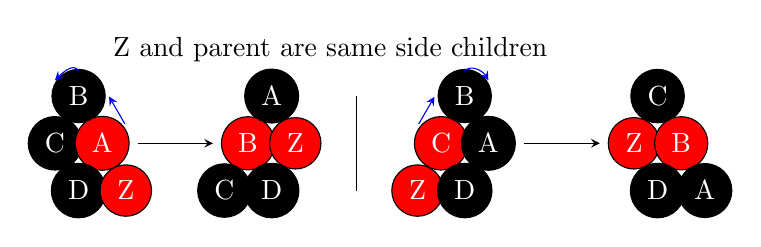
\begin{tikzpicture}[
            scale=0.4,
            blk/.style ={
                circle,
                white,
                fill=black,
                draw=black
            },
            rd/.style ={
                circle,
                white,
                fill=red,
                draw=black
            }
            ]
            \node[blk] (grandparent) at (0,0) {B}
                child{node[blk] (uncle) {C}}
                child{node[rd] (parent) {A}
                    child{node[blk] (sib) {D}}
                    child{node[rd] (self) {Z}}
                };
            \path[->,blue] ($(grandparent)+(0,0.8)$) edge [in=45,out=120] ($(grandparent)+(-0.75,0.5)$);
            \path[->,blue] ($(parent.north east)+(0.1,0)$) edge +(120:1);
            \node () [above right=1mm of grandparent] {Z and parent are same side children};
            \node[blk] (agrandparent) [right=5em of grandparent] {A}
                child{node[rd] (aparent) {B}
                    child{node[blk] (asib) {C}}
                    child{node[blk] (aself) {D}}
                }
                child{node[rd] (auncle) {Z}};
            \path[->] (parent.east) ++(0.25,0) edge ($(aparent.west)+(-0.25,0)$);

            %% Mirrored

            \node[blk] (mgrandparent) [right=5em of agrandparent] {B}
                child{node[rd] (muncle) {C}
                    child{node[rd] (mself) {Z}}
                    child{node[blk] (msib) {D}}
                }
                child{node[blk] (mparent) {A}};
            \path[->,blue] ($(mgrandparent)+(0,0.8)$) edge [in=120,out=45] ($(mgrandparent)+(0.75,0.5)$);
            \path[->,blue] ($(muncle.north west)+(-0.1,0)$) edge +(60:1);
            \node[blk] (magrandparent) [right=5em of mgrandparent] {C}
                child{node[rd] (maparent) {Z}}
                child{node[rd] (mauncle) {B}
                    child{node[blk] (maself) {D}}
                    child{node[blk] (masib) {A}}
                };
            \path[->] (mparent.east) ++(0.25,0) edge ($(maparent.west)+(-0.25,0)$);

            %% Anti-confusion mirror line
            \draw[draw] let \p1 = ($(auncle)!0.5!(mself)$),
                \p2 = (maself) in ($(\x1,0)$) -- +(0,\y2);
            %% Above line is overly complicated for what it is

        \end{tikzpicture}%
        }
\end{enumerate}

\subsubsection*{Deletion}

DB node has\ldots
\begin{enumerate}%
    \item {\bfseries\color{black}black sibling with at least one red child.}
        This fixes the problem structurally. No extra work is required
        after this case completes. This corresponds to a transfer operation in a 2-4 Tree.
    \item {\bfseries\color{black}black sibling with two black children.}
        This uses recoloring and no structural change. It may solve the problem, but
        may ALSO propagate the DB node to the parent of the current DB node. This corresponds
        to a fusion and drop operation in a 2-4 Tree.
    \item {\bfseries\color{black}red sibling.}
        A structural change here puts you in case 1 or case 2.
        At this point, a single application of either case is sufficient.
        This corresponds to a fusion where you have enough values in the parent node to drop
        one into the fused child.
\end{enumerate}

\subsection*{Skip Lists}
Stacks of linked lists.
\subsubsection*{Insertion}
Insert at bottom level. 50\% chance it's added up, again \& again. Stop if it is only one at top level.
\subsubsection*{Deletion}
Delete value and update all pointers.
%TODO: More Info

    \section{Algorithm Analysis}
{\scriptsize $\lg n=\log_2n$}
\subsection*{Order Notation}
\subsubsection*{Big-Oh ($O$)}
Big-Oh is an upper bound. It simply guarantees that a function is no larger than a constant times a function $g(n)$, for $O(g(n))$.

$f(n)=O(g(n))\textrm{ iff }\forall n\ge n_0$ \footnotesize{(const $n_0$)}

$f(n)\le cg(n)\ \textrm{for some const } c$

\subsubsection*{Big-Omega ($\Omega$)}
$f(n)=\Omega(g(n))\textrm{ iff }\forall n\ge n_0$ \footnotesize{(const $n_0$)}

$f(n)\ge cg(n)\ \textrm{for some const } c$

\subsubsection*{Big-Theta ($\Theta$)}
$f(n)=\Theta(g(n))\ \textrm{iff}\ f(n)=O(g(n))\\ \textrm{and}\ f(n)=\Omega(g(n))$

$f(n)=\Theta(g(n))\\%
\textrm{iff}\ \lim_{n\to\infty}\frac{f(n)}{g(n)}>0${\color{myblue},}
{\scriptsize\color{myblue}where const $c$ and $c>0$}

\subsection*{Master Theorem}
$T(n)=\overbrace{A}^{\mathclap{\textrm{\# of sub probs in recursion}}}T\underbrace{\bigl(\frac{n}{B}\bigr)}_{\mathclap{\textrm{size of ea. sub problem}}}%
+\overbrace{O(n^k)}^{\mathrlap{\subalign{\text{c}&\text{ost of work done}\\\text{o}&\text{ut of recursive call}}}}$

\resizebox{.75\linewidth}{!}{%
$T(n)=\begin{cases}%
B^k<A\Rightarrow O(n^{\log{B^A}})\\%
B^k=A\Rightarrow O(n^{k}\lg{n})\\%
B^k>A\Rightarrow O(n^{k})\\%
\end{cases}$}
\subsection*{Expectation Definition}
$E(x)=\sum_{x\in X}x\cdot p(x)$
\subsection*{Binomial Theorem}
${\left(x+y\right)}^n=\sum_{k=0}^n\binom{n}{k}x^{k}y^{n-k}$

$\overbrace{\binom{n}{k}}^{\mathrlap{\textrm{\# of ords of }k\textrm{ suc }n-k\textrm{ fail}}}%
\underbrace{p^k}_{\mathrlap{\textrm{prob of k suc in their slots}}}%
\overbrace{{\left(1-p\right)}^{n-k}}^{\mathrlap{\textrm{\raisebox{-.3\normalbaselineskip}[0pt][0pt]{same for fails}}}}$
\subsection*{Binary Search Average Case Run Time}
$O(\log n)$ % TODO: Show Math
\subsection*{Make Heap Worst Case Run Time}
$O(n\log n)$
% TODO: Pic from review: https://cdn.discordapp.com/attachments/967445734842585088/968622073490587668/IMG_7722.jpg
\subsection*{Quick Select Average Case Run Time}
$O(n)$

    \section{Sorting}
\subsection*{Lower Bounds}

\subsubsection*{Comparison Sorts}
% https://www.cs.ucf.edu/~dmarino/ucf/cop3503/lectures/MoreSorting01.pdf#page=5

Given an input of n numbers to sort, they can be arranged in $n!$ different orders.
With $k$ cols, each with 2 possible answers, there are $2^k$ possible distinct rows.
$\Omega(n\log n)$

\resizebox{\linewidth}{!}{%
\begin{tabular}{@{} ccccc @{}}
    Input & $a[1]>a[2]$ & $a[1]>a[3]$ & $a[2]>a[3],\dots$ & $a[n-2]>a[n-1]$\\
    2,1,4,3 & T & F & F & T\\
    2,3,1,4 & F & T & T & F\\
    4,3,2,1 & T & T & T & T
\end{tabular}
}

\subsubsection*{Adjacent Element Swap Sorts}
% https://www.cs.ucf.edu/~dmarino/ucf/cop3503/lectures/MoreSorting01.pdf#page=4

An inversion in a list of numbers is a pair of numbers that are out of order relative to each other.

The average number of inversions in a random list of distinct numbers is:

$\frac{1}{2}\binom{n}{2}=\frac{n(n-1)}{2}=\Omega(n^2)$

The average case run-time of all of these algorithms is $\Omega(n^2)$.


\subsection*{Bucket Sort}
Inputs randomly distributed in range $\left[x,N\right)$, for n amount of values, create different buckets to hold the values. $\frac{N}{n}$ will give the new ranges. $O(n)$

Consider sorting a list of 10 numbers known to be in between 0 and 2, not including 2 itself. Thus, each bucket will store values in a range of $\frac{2}{10}=.2$ In particular, we have the following list:

\begin{tabularx}{\linewidth}{XX}
    Bucket & Range of Values\\
    \toprule
    0 & $\left[0,.2\right)$ \\
    1 & $\left[.2,.4\right)$ \\
    2 & $\left[.4,.6\right)$ \\
    3 & $\left[.6,.8\right)$ \\
    4 & $\left[.8,1\right)$ \\
    5 & $\left[1,1.2\right)$ \\
    6 & $\left[1.2,1.4\right)$ \\
    7 & $\left[1.4,1.6\right)$ \\
    8 & $\left[1.6,1.8\right)$ \\
    9 & $\left[1.8,2\right)$
\end{tabularx}

\subsection*{Counting Sort}

In counting sort, each of the values being sorted are in the range from 0 to m, inclusive.
Here is the algorithm for sorting an array a[0],\dots,a[n-1]:

\begin{enumerate}
    \item Create an aux c, indexed from $c[0]$ to $c[m]$ and init each value in the array to 0.
    \item Run through the input array a, tabulating the number of occurrences of each
        value 0 through m by adding 1 to the value stored in the appropriate index in c.
        (Thus, c is a freq array.)
    \item Run through the array c, a \nth{2} time so that the value stored in each
        array slot represents the number of elements $\le$ the index value in the
        original array a.
    \item Now, run through the original input array a, and for each value in a, use
        the aux array c to tell you the proper placement of that value in the sorted
        input, which will be stored in a new array $b[0]..b[n-1]$.
    \item Copy the sorted array from b to a.
\end{enumerate}

% TODO: Add example maybe?

\subsection*{Radix Sort}

input: non-neg ints, k digits long, $O(nk)$.

\begin{enumerate}
    \item Sort the values using a $O(n)$ stable sort on the kth most sig.\ digit.
    \item Decrement k by 1
    \item Repeat step 1. (Unless $k=0$, then you're done.)
\end{enumerate}

\begin{tabular}{cccc}
    unsorted & $v_1$ & $v_2$ & $v_3$\\
    \toprule
    235 & 162 & 628 & 162\\
    162 & 734 & 734 & 175\\
    734 & 674 & 235 & 235\\
    175 & 235 & 237 & 237\\
    237 & 175 & 162 & 628\\
    674 & 237 & 674 & 674\\
    628 & 628 & 175 & 734
\end{tabular}

$v_1$: sorted by units digit

$v_2$: sorted by tens digit

$v_3$: sorted by hundreds digit

    \section{Greedy Algorithms}
\subsection*{Fractional Knapsack}
Goal is to maximize the value of a knapsack that can hold at most $W$ units worth
of goods from a list of items $I_1,I_2, \dots I_n$.

Each item has 2 attrs:
\begin{enumerate}
    \item A value/weight; let this be $v_i$ for item $I_i$.
    \item Weight available; let this be $w_i$ for item $I_i$.
\end{enumerate}
The algorithm is as follows:
\begin{enumerate}
    \item Sort the items by value/unit.
    \item Take as much as you can of the most expensive item left,
        moving down the sorted list. You may end up taking a fractional portion
        of the "last" item you take.
\end{enumerate}
\subsection*{Single Room Scheduling}
Given a single room to schedule, and a list of requests, the goal of this problem
is to maximize the total number of events scheduled.
Each request simply consists of the group, a start time and an end time during the day.

Here's the greedy solution:
\begin{enumerate}
    \item Sort the requests by finish time.
    \item Go through the requests in order of finish time,
        scheduling them in the room if the room is unoccupied at its start time.
\end{enumerate}
\subsection*{Multiple Room Scheduling}
Given a set of requests with start and end times, the goal here is to schedule
all events using the minimal number of rooms.
Once again, a greedy algorithm will suffice:
\begin{enumerate}
    \item Sort all the requests by start time.
    \item Schedule each event in any available empty room.
        If no room is available, schedule the event in a new room.
\end{enumerate}
\subsection*{Change}
The goal here is to give change with the minimal number of coins possible for a
certain number of cents using 1 cent, 5 cent, 10 cent, and 25 cent coins.

The greedy algorithm is to keep on giving as many coins of the
largest denomination until you the value that remains to be
given is less than the value of that denomination. Then you
continue to the lower denomination and repeat until you've
given out the correct change.
\subsection*{Huffman Coding}
For the following character frequencies:

\begin{tabular}{cc}
    Character & Frequency \\
    a & 12\\
    b & 2\\
    c & 7\\
    d & 13\\
    e & 14\\
    f & 85
\end{tabular}

Create a binary tree for each char that also stores the frequency w/ which it occurs.

\columnbreak[0]
The algorithm is as follows:
\begin{enumerate}
    \item Find the two bin trees in the list that store min freqs at their nodes.
    \item Connect these two nodes at a newly created common node that will store NO
        character but will store the sum of the freqs of all nodes connected below it.
\end{enumerate}

\resizebox{\linewidth}{!}{%
\begin{tikzpicture}[
    scale=0.4,
    node/.style ={
        rectangle,
        fill=white,
    },
    pics/n/.style args={#1/#2}{
        code={
            \node[node] (#2) {#1 '#2'};
        }
    }
    ]
    \node (9) {$9$}
        child{pic{n=2/b}}
        child{pic{n=7/c}};
    \pic[right=of 9]{n=12/a};
    \pic[right=of a]{n=13/d};
    \pic[right=of d]{n=14/e};
    \pic[right=of e]{n=85/f};
\end{tikzpicture}
}

Repeat until only one tree is left:

\resizebox{\linewidth}{!}{%
\begin{tikzpicture}[
    scale=0.4,
    level/.style={sibling distance=40em/#1},
    node/.style ={
        rectangle,
    },
    ]
    \node[node] (133) {133}
        child{
            node (48) {48}
                child{
                    node (21) {21}
                        child{
                            node (9) {9}
                                child{node[node] (b) {2 'b'}}
                                child{node[node] (c) {7 'c'}}
                        }
                        child{node[node] (a) {12 'a'}}
                }
                child{
                    node (27) {27}
                        child{node[node] (d) {13 'd'}}
                        child{node[node] (e) {14 'e'}}
                }
        }
        child{node[node] (f) {85 'f'}};

\end{tikzpicture}
}

One the tree is built, each leaf node corresponsds to a letter w/ a code.
To determine the code for a node, walk a std search path from the root to the leaf node.

For every step to the left, append a 0 to the code and for every step right, append a 1.

For the ex.\ tree we get the codes:

\begin{tabular}{cc}
    Character & Code \\
    a & 001\\
    b & 0000\\
    c & 0001\\
    d & 010\\
    e & 011\\
    f & 1
\end{tabular}
\subsubsection*{Calculating Bits Saved}
$\text{total bits}=\sum \text{char}_{\text{freq}}\cdot \text{char}_{\text{\# bits}}=\\%
\left(12\cdot 3\right)_{a}+\cdots+\left(85\cdot 1\right)_{f}=238$

Assuming the original file is storing each of the 6 chars with a 3-bit code.
Since there are 133 such characters, the total num of bits used before huffman is $3\cdot 133=399$.

$\therefore$ we saved $399 - 238 = 161$ bits.

    \section{Unweighted Graphs}
\subsection*{Types}
\resizebox{\linewidth}{!}{%
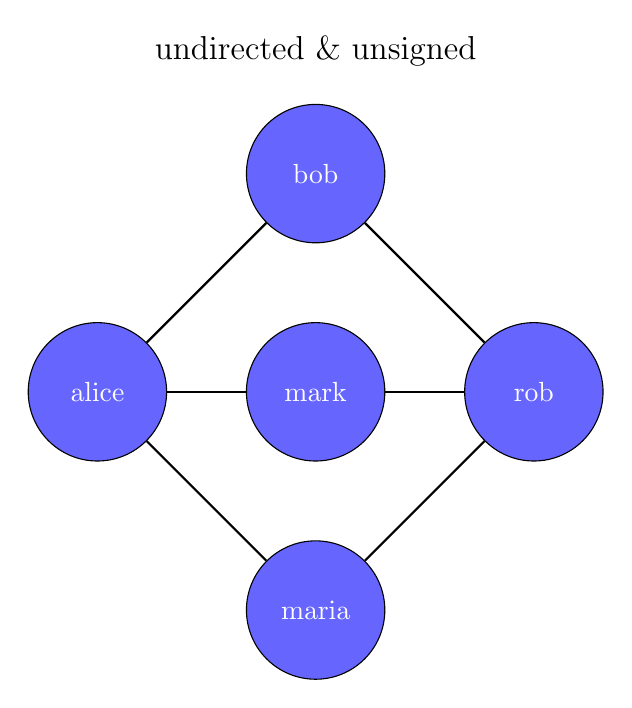
\begin{tikzpicture}[
    p/.style ={
        minimum size=5em,
        circle,
        white,
        fill=blue!60,
        draw=black
    }
    ]

    \node[p] (bob) {bob};
    \node () [above=1em of bob] {\large undirected \& unsigned};
    \node[p] (mark) [below=of bob] {mark};
    \node[p] (alice) [left=of mark] {alice};
    \node[p] (rob) [right=of mark] {rob};
    \node[p] (maria) [below=of mark] {maria};

    \foreach \src/ \dst in {bob/alice, rob/bob, mark/alice, rob/mark, alice/maria, rob/maria}
        \path[draw,thick] (\src) -- (\dst);
\end{tikzpicture}
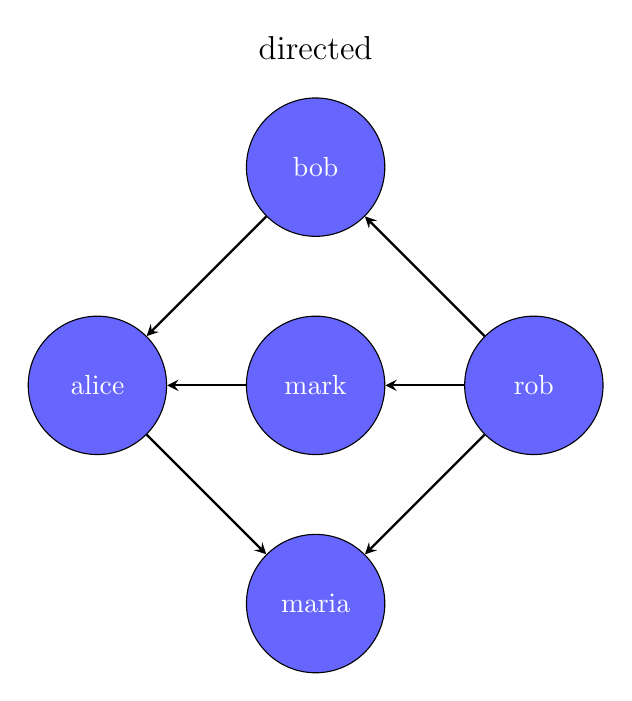
\begin{tikzpicture}[
    p/.style ={
        minimum size=5em,
        circle,
        white,
        fill=blue!60,
        draw=black
    }
    ]

    \node[p] (bob) {bob};
    \node () [above=1em of bob] {\large directed};
    \node[p] (mark) [below=of bob] {mark};
    \node[p] (alice) [left=of mark] {alice};
    \node[p] (rob) [right=of mark] {rob};
    \node[p] (maria) [below=of mark] {maria};

    \foreach \src/ \dst in {bob/alice, rob/bob, mark/alice, rob/mark, alice/maria, rob/maria}
        \path[->,thick] (\src) edge (\dst);
\end{tikzpicture}
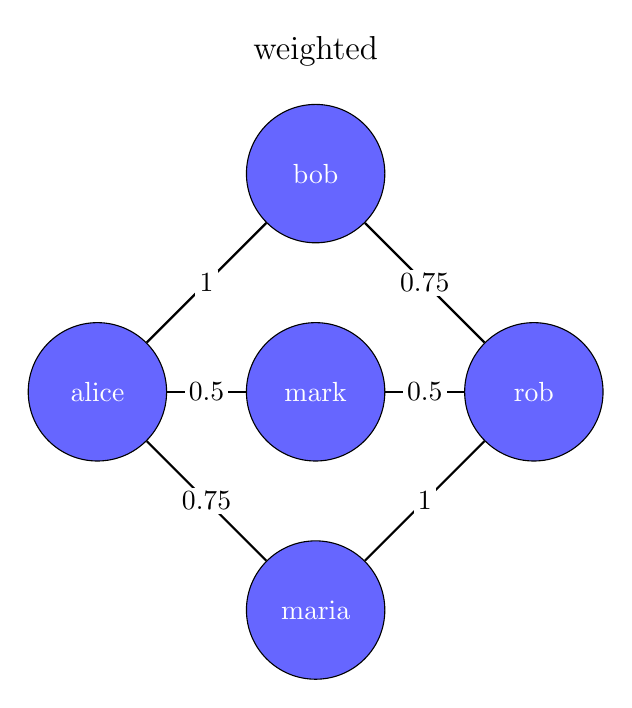
\begin{tikzpicture}[
    p/.style ={
        minimum size=5em,
        circle,
        white,
        fill=blue!60,
        draw=black
    },
    inside/.style ={
        midway,
        fill=white,
        inner sep=1.5pt,
        outer sep=2pt
    }
    ]

    \node[p] (bob) {bob};
    \node () [above=1em of bob] {\large weighted};
    \node[p] (mark) [below=of bob] {mark};
    \node[p] (alice) [left=of mark] {alice};
    \node[p] (rob) [right=of mark] {rob};
    \node[p] (maria) [below=of mark] {maria};

    \foreach \src/ \dst/ \weight in {bob/alice/1, rob/bob/0.75, mark/alice/0.5, rob/mark/0.5, alice/maria/0.75, rob/maria/1}
        \draw[draw,thick] (\src) -- node[inside] {\weight} (\dst);
\end{tikzpicture}
}

\subsection*{Depth First Search}
Search down a path from a vertex as far as you can go. Then backtrack to the last vertex from which a different path could have been taken. $O(V+E)$

\subsection*{Breadth First Search}
Search all the paths at a uniform depth from the source before moving into deeper paths.

\subsection*{Topological Sort}
Can find a top.\ ord.\ in $O(V+E)$ time.

\subsubsection*{Topological Ordering}
An ordering of the nodes in a directed graph where for each directed edge from node A to node B,
node A appears before node B in the ordering.

Top.\ ords.\ are NOT unique.

%\vspace{1em}! % Fixes clipping issue with "Top. ..." text

%\newcolumn
A graph which contains a cycle cannot have a valid ordering:

\resizebox{.5\linewidth}{!}{%
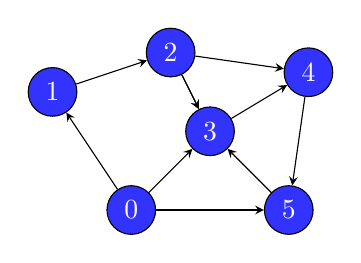
\begin{tikzpicture}[
    n/.style ={
        circle,
        white,
        fill=blue!80,
        draw=black
    }
    ]
    \foreach \x/ \pos in {{0/(1,0)}, {1/(0,1.5)}, {2/(1.5,2)}, {3/(2,1)}, {4/(3.25,1.75)}, {5/(3,0)}}
        \node[n] (\x) at \pos {\x};

    \foreach \src/ \dst in {0/1, 1/2, 2/3, 0/3, 0/5, 3/4, 2/3, 2/4, 4/5, 5/3}
        \draw[->] (\src) -- (\dst);

\end{tikzpicture}
}

The only type of graph which has a valid top.\ ordering is a {\bfseries Directed Acyclic Graph (DAG)}.
These are graphs with directed edges and no cycles.

ie: Program dependency graph.

\resizebox{\linewidth}{!}{%
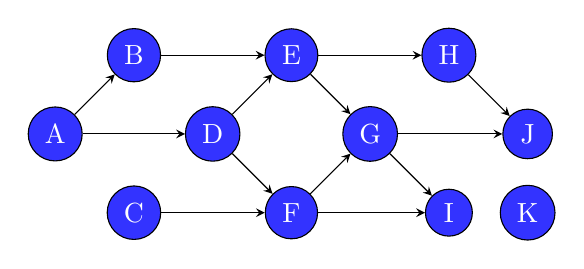
\begin{tikzpicture}[
    n/.style ={
        circle,
        white,
        fill=blue!80,
        draw=black
    }
    ]
    \foreach \x/ \pos in {{A/(0,1)}, {B/(1,2)}, {C/(1,0)}, {D/(2,1)}, {E/(3,2)},
                          {F/(3,0)}, {G/(4,1)}, {H/(5,2)}, {I/(5,0)}, {J/(6,1)},
                          {K/(6,0)}}
        \node[n] (\x) at \pos {\x};

    \foreach \src/ \dst in {A/B, A/D, B/E, D/E, D/F, C/F, E/G, E/H, F/G, F/I, G/I, G/J, H/J}
        \draw[->] (\src) -- (\dst);

\end{tikzpicture}
}

\subsubsection*{Topological Algorithm}
\begin{enumerate}
    \item Pick an unvisited node
    \item Beginning w/ the selected node, do a DFS exploring only unvisited nodes.
    \item On the recursive callback of the DFS, add the current node to the top.\ ordering in rev.\ order.
\end{enumerate}


    \section{Weighted Graphs}
\subsection*{Dijkstra's}
Finds the shortest path from a src vertex to all other vertices in a weighted
directed graph w/out negative edge weights. (uses BFS)

\subsubsection*{Dijkstra's Trace}

\resizebox{.5\linewidth}{!}{%
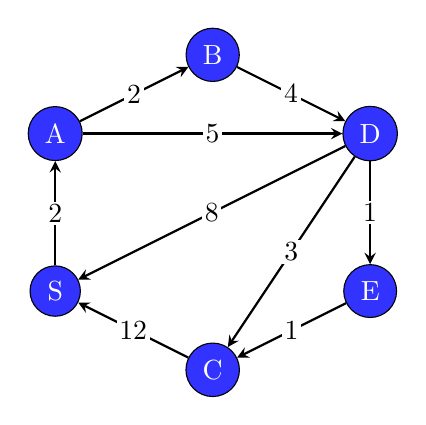
\begin{tikzpicture}[
    n/.style ={
        circle,
        white,
        fill=blue!80,
        draw=black
    },
    inside/.style ={
        midway,
        fill=white,
        inner sep=1pt,
        outer sep=1pt
    }
    ]
    \foreach \x/ \pos in {{A/(0,2)}, {B/(2,3)}, {C/(2,-1)}, {D/(4,2)}, {E/(4,0)},
                          {S/(0,0)}}
        \node[n] (\x) at \pos {\x};

    \foreach \src/ \dst/ \weight in {S/A/2, A/B/2, B/D/4, A/D/5, D/S/8, D/C/3, D/E/1, E/C/1, C/S/12}
        \draw[->,thick] (\src) -- node[inside] {\weight} (\dst);
\end{tikzpicture}
}

\begin{tabular}{@{} ccccccc @{}}
     & \multicolumn{6}{c}{Distances}\\
    {\scriptsize processed} & S & A & B & C & D & E\\
    \toprule
      & 0 & $\infty$ & $\infty$ & $\infty$ & $\infty$ & $\infty$ \\
    S (0) & 0 & 2 & $\infty$ & 12 & 8 & $\infty$ \\
    A (2) & 0 & 2 & 4 & 12 & 7 & $\infty$ \\
    B (4) & 0 & 2 & 4 & 12 & 7 & $\infty$ \\
    D (7) & 0 & 2 & 4 & 10 & 7 & 8\\
    E (8) & 0 & 2 & 4 & 9 & 7 & 8\\
    C (9) & 0 & 2 & 4 & 9 & 7 & 8
\end{tabular}

\subsection*{Minimum Spanning Trees}

\bold{tree:} A connected graph w/out cycles.

\bold{Spanning Tree:} A subtree of a graph that includes each vertex of the graph.
A subtree of a given graph as a subset of the components of that given graph.

\bold{Minimum Spanning Tree:} Only def for weighted graphs.
This is the spanning tree of a given graph whose $\sum\text{edge weights}$ is min, compared
to all other spanning trees.

%\vspace{1em}! % Fixes clipping issue with "min span tree" par


\resizebox{\linewidth}{!}{%
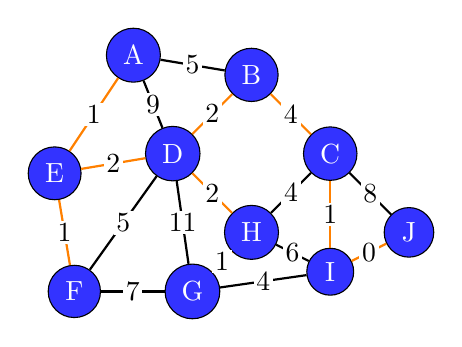
\begin{tikzpicture}[
    n/.style ={
        circle,
        white,
        fill=blue!80,
        draw=black
    },
    inside/.style ={
        midway,
        fill=white,
        inner sep=1pt,
        outer sep=1pt
    }
    ]
    \foreach \x/ \pos/ \sel in {{A/(1,3)/black}, {B/(2.5,2.75)/black}, {C/(3.5,1.75)/black}, {D/(1.5,1.75)/black},
                                {E/(0,1.5)/black}, {F/(0.25,0)/black}, {G/(1.75,0)/black}, {H/(2.5,0.75)/black},
                                {I/(3.5,0.25)/black}, {J/(4.5,0.75)/black}}
        \node[n] (\x) at \pos {\x};

    \foreach \src/ \dst/ \weight/ \sel in {E/F/1/orange, E/A/1/orange, E/D/2/orange, F/D/5/black, A/D/9/black, A/B/5/black,
                                     D/B/2/orange, F/G/7/black, G/D/11/black, G/H/1/orange, G/I/4/black, D/H/2/orange,
                                     H/I/6/black, H/C/4/black, B/C/4/orange, C/J/8/black, I/C/1/orange, I/J/0/orange}
        \draw[draw,thick,\sel] (\src) -- node[inside] {\color{black}\weight} (\dst);
\end{tikzpicture}
}
{\scriptsize ({\color{orange}orange}) Minimum spanning tree with weight 14}

\subsection*{Kruskal's}
\begin{enumerate}
    \item Sort edges by ascending edge weight.
    \item Walk through the sorted edges and look at the two nodes the edge belongs
        to, if the nodes are already unified we don't include this edge, otherwise
        we include it and unify the nodes.
    \item The algorithm terminates when every edge has been processe or all the vertices
        have been unified.
\end{enumerate}

%Let $V=\emptyset$

%For $i=1\to n-1$, (where there are n vertices in a graph)

%$V=V\cup e$, where $e$ is the edge w/ the min edge weight $\notin V$, and that does NOT form a
%cycle when added to $V$.

%Return $V$

\subsection*{Prim's}

A greedy MST algorithm that works well on dense graphs.
However, when finding the minimum spanning forest on a disconnected graph,
Prim's must be run on each connected component individually.

The lazy version of Prim's has a runtime of $O(E\log E)$, and the eager version
has a better runtime of $O(E\log V)$.

\subsubsection*{Lazy Prim's}

\begin{enumerate}
    \item Maintain a min Priority Queue that sorts edged based on min edge cost.
    \item Start the algorithm on any node \bold{s}. Mark \bold{s} as visited and iterate
        over all edges of \bold{s}, adding them to the PQ.
    \item While the PQ is not empty and a MST has not been formed, dequeue the next cheapest
        edge from the PQ.
        If the dequeued edge has already been visited, skip it and poll again.
        Otherwise, marked the current node as visited and add the selected edge to the MST.
    \item Iterate over the new current node's edges and all all its edges to the PQ.
        Do not add edges to the PQ which point to already visited nodes.
\end{enumerate}

\begin{lstlisting}[language=Java,basicstyle=\tiny]
// edge implements Comparable
public ArrayList<edge> prims(
  ArrayList<edge>[] graph
) {
  int n = graph.length;
  // shortened to PQ for spacing
  PQ<edge> pq = new PriorityQueue<edge>();
  boolean[] used = new boolean[n];
  used[0] = true;
  for (edge e: graph[0])
    pq.offer(e);

  ArrayList<edge> mst = new ArrayList<edge>();
  while (pq.size() > 0 && mst.size() < n-1) {
    edge cur = pq.poll();
    if (used[cur.u] && used[cur.v]) continue;
    int newV = !used[cur.u] ? cur.u : cur.v;
    mst.add(cur);

    used[newV] = true;
    for (edge e: graph[newV])
      pq.offer(e);
  }
  if (mst.size() < n-1) return null;
  return mst;
}
\end{lstlisting}

%\begin{enumerate}
    %\item Set $S=\emptyset$.
    %\item Pick any vertex in the graph.
    %\item Add the min edge incident to that vertex to S.
    %\item Continue to add edges into S (n-2 more times) using the following rule:
        %Add the min edge weight to S that is incident to S but that doesn't form
        %a cycle when added to S.
%\end{enumerate}

\subsection*{Network Flow}

\bold{Max-Flow, Min-Cut Theorem:} The value of the maximal flow in a flow network
equals the value of the minimum cut.

\subsubsection*{Ford Fulkerson}
While there exists an augmenting path:
Add the appropriate flow to that augmenting path.

Typically, DFS is used to check for the existence of an augmenting path.

worse-case, the algorithm takes $O(|f|E)$ time, where $|f|$ is the maximal flow  of the network.

\subsubsection*{Edmonds Karp Algorithm}
A variation on the Ford-Fulkerson method. Idea is to stry to choose good augmenting paths.
In this algorithm, the augmenting path suggested is the augmenting path with the mininal
number of edges. (Can be found using BFS) The total number of iters is $O(VE)$. Thus,
total run time with the graph stored as an adj.\ matrix is $O(V^3E)$.


\subsubsection*{Dinic's Algorithm}
A strongly polynomial max flow algorithm with a runtime of $O(V^2E)$.

The strongly polynomial means that the runtime does not depend on the capacity
values of the flow graph.

Extremely fast and works even better on bipartite graphs, with a time complexity
of $O(\sqrt{V}E)$ due to the algorithm's reduction to Hopcroft-Karp.

The main idea is to guide augmenting paths from $s\to t$ using a level graph.

\subsubsection*{Level Graph}

An edge is only part of the level graph if it makes progress towards the sink.
That is, the edge must go from a node at Level $L$ to another at level $L+1$.

\resizebox{\linewidth}{!}{%
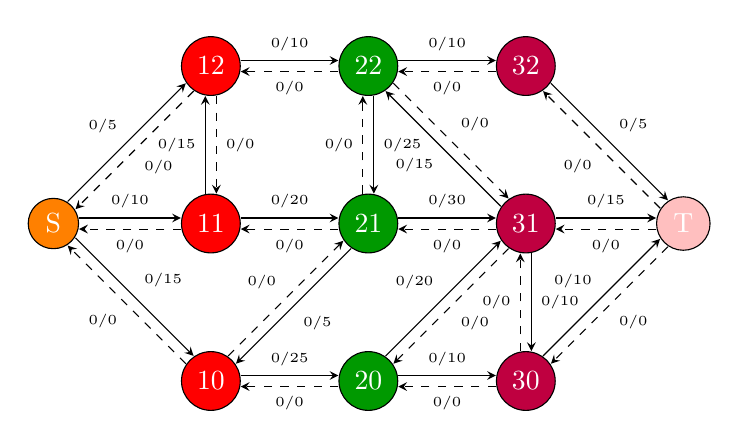
\begin{tikzpicture}[
    auto,
    scale=2,
    n/.style ={
        circle,
        white,
        fill=blue!80,
        draw=black
    },
    inside/.style ={
        midway,
        fill=white,
        inner sep=1pt,
        outer sep=1pt
    }
    ]
    \foreach \x/ \y/ \pos/ \clr in {{S//(0,1)/orange}, {1/0/(1,0)/red}, {1/1/(1,1)/red}, {1/2/(1,2)/red},
                                {2/0/(2,0)/codegreen}, {2/1/(2,1)/codegreen}, {2/2/(2,2)/codegreen},
                                {3/0/(3,0)/purple}, {3/1/(3,1)/purple}, {3/2/(3,2)/purple}, {T//(4,1)/pink}}
        \node[n,fill=\clr] (\x\y) at \pos {\x\y};

    \foreach \src/ \dst/ \fwd/ \bck in {
        S/10/{0/15}/{0/0}, S/11/{0/10}/{0/0}, S/12/{0/5}/{0/0}, 11/12/{0/15}/{0/0},
        21/10/{0/5}/{0/0}, 10/20/{0/25}/{0/0}, 11/21/{0/20}/{0/0}, 12/22/{0/10}/{0/0},
        22/21/{0/25}/{0/0}, 31/22/{0/15}/{0/0}, 22/32/{0/10}/{0/0}, 21/31/{0/30}/{0/0},
        20/30/{0/10}/{0/0}, 20/31/{0/20}/{0/0}, 31/30/{0/10}/{0/0}, 32/T/{0/5}/{0/0},
        31/T/{0/15}/{0/0}, 30/T/{0/10}/{0/0}}{
        \path[->,dashed] let \p1=($(\src)-(\dst)$), \n1={atan2(\y1, \x1)}, \n2={180+\n1} in
            ($ (\dst.\n1)!1pt!90:(\src.\n2) $) edge node {\tiny \bck} ($ (\src.\n2)!1pt!-90:(\dst.\n1) $);
        \path[->] let \p1=($(\dst)-(\src)$), \n1={atan2(\y1, \x1)}, \n2={180+\n1} in
            ($ (\src.\n1)!1pt!90:(\dst.\n2) $) edge node {\tiny \fwd} ($ (\dst.\n2)!1pt!-90:(\src.\n1) $);
        %\draw[<->,thick] (\src) -- (\dst);
    };
\end{tikzpicture}
}

% TODO: Finish example: https://youtu.be/M6cm8UeeziI?t=347

Algorithm Steps:

\begin{enumerate}
    \item Construct a level graph by doing a BFS from the src to label all the levels
        of the current flow graph.
    \item If the sink was never reached while building the level graph, then stop and
        return the max flow.
    \item Using only valid edges in the level graph, do multiple DFSs from $s\to t$ until a
        blocking flow is reached, and sum over the bottleneck values of all the
        augmenting paths found to calculate the max flow.
    \item Repeat Steps $1\to 3$
\end{enumerate}

% If have room, may add Bipartite Matching:
% http://www.cs.ucf.edu/~dmarino/ucf/cop3503/lectures/NetworkFlow.pdf#page=7

    \section{Divide and Conquer}
\subsection*{Integer Multiplication}

Imagine multiplying an n-bit number by another n-bit
number, where n is a perfect power of 2.
(This will make the analysis easier.)
We can split up each of these numbers into two halves. 

$I\times J=[(I_h\times 2^{\frac{n}{2}}+I_l)]\times[(J_h\times 2^{\frac{n}{2}}+J_l)]=%
I_h\times J_h\times 2^n+(I_l\times J_h+I_h\times J_l)\times 2^{\frac{n}{2}}+I_l\times J_l$

This way, we have broken down the problem of 2 n-bit nums into 4 mults of
n/2-bit nums plus 3 addtions.
Thus the run-time $T(n)=4T(n/2)+\theta(n)$

This has the solution of $T(n)=\theta(n^2)$ by the Master Theorem.

To optimize this:

$P_1=(I_h+I_l)\times(J_h+J_l)=I_h\times J_h+I_x\times J_l+I_l\times J_h+I_l\times J_l$


$P_2=I_h\times J_h$

$P_3=I_l\times J_l$

$P_1-P_2-P_3=I_h\times J_1+I_l\times J_h$

$I\times J=P_2\times 2^n+[P_1-P_2-P_3]\times 2^{\frac{n}{2}}+P_3$

\subsection*{Tromino "Tiling"}
A tromino is a figure composed of three 1x1 squares in the shape of an L.
Given a $2^n\times 2^n$ checkerboard with 1 missing square, we can recursively tile that 
square with trominoes.

\begin{enumerate}
    \item Split the board into four equal sized squares.
    \item The missing square is in one of these four squares.
        Recursively tile this square since it is a proper recursive case.
    \item Although the three other squares aren't missing squares, we can "create"
        these recursive cases by tiling one tronimo in the center of the board,
        where appropriate:
\end{enumerate}

\resizebox{\linewidth}{!}{%
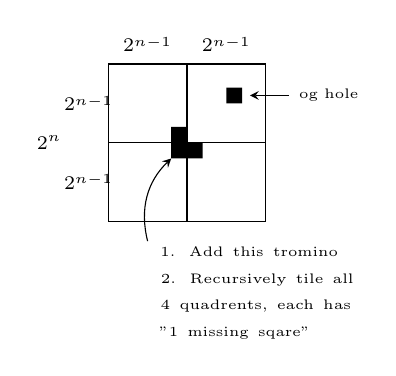
\begin{tikzpicture}

    \foreach \x/ \y in {0.5/2.25, 1.5/2.25, -0.25/0.5, -0.25/1.5} {
        \node () at (\x,\y) {\scriptsize $\cramped{2^{n-1}}$};
    };

    \node () at (-0.75,1) {\scriptsize $2^n$};

    \path[draw] (0,0) rectangle ++(2,2)
        (1,0) -- +(0,2)
        (0,1) -- +(2,0);

    \path[<-,fill]
        % o.g. hole
        (1.5,1.5) rectangle ++(0.2,0.2)
        ++(0.1,-0.1) edge +(.5,0) ++(0.5,0) node[right] () {\tiny og hole}
        (1,1) rectangle ++(-0.2,0.2)
        (1,1) rectangle ++(0.2,-0.2)
        (1,1) rectangle ++(-0.2,-0.2)
        edge[bend right=30] (0.5,-0.25) ++(-0.25,-1) node[below right,text width=7em] () {\tiny 1. Add this tromino\\ 2. Recursively tile all 4 quadrents, each has "1 missing sqare"};
\end{tikzpicture}
}

\subsection*{Skyline Problem}
\lipsum[1][1-2]
\subsection*{Closest Pair of Points}
The Closest Pair of Points Algorithm is an O(nlogn) solution to the problem of finding the closest pair of points
when given a set of points with (x,y) coordinates. It has a base case of 2 points and a second base case of 3 points.
Base case size 3 uses a brute force algorithm to return the closest pair. Base case size 2 returns that the distance between the two points.
\begin{enumerate}
    \item Sort the points based on their x coordinates (Use merge or quick)
    \item Recursively split the sorted array in halves (like a merge sort does) until the base case of 3 or 2 is met.
    \item To merge the halves, find the minimum distance out of the two halves, and label it delta. 
    \item Create an Array of all of the points within 'delta' distance of the halfway line.
    \item Sort this array based on the y coordinates (use merge or quick).
    \item Brute force search for the smallest distance within this array (Max size of array is 8) 
    \item This smallest distance is the true smallest distance for this section. Repeat the process.
\end{enumerate}
\subsection*{Strassen's Algorithm}
\lipsum[1][1-2]

    \section{Dynamic Programming}
\subsection*{Fibonacci}
\lipsum[1][1-2]
\subsection*{Combinations}
\lipsum[1][1-2]
\subsection*{Longest Common Subsequence (LCS DP)}
\lipsum[1][1-2]
\subsection*{Number of Ways to Make Change}
\lipsum[1][1-2]
\subsection*{Fewest Number of Coins to Make Change}
\lipsum[1][1-2]
\subsection*{0-1 Knapsack Problem}
\lipsum[1][1-2]
\subsection*{Floyd-Warshall's Algorithm and path reconstruction}
\lipsum[1][1-2]
\subsection*{Matrix Chain Multiplication}
\lipsum[1][1-2]
\subsection*{Edit Distance}
\lipsum[1][1-2]
\subsection*{Road Optimization Problem Idea}
\lipsum[1][1-2]

    \section{Probabilistic Algorithms}
\subsection*{Fermat's Theorem}
\lipsum[1][1-2]
\subsection*{Miller-Rabin Primality Test}
\lipsum[1][1-2]
\subsection*{Rolling Hash Function and String Matching}
\lipsum[1][1-2]

\end{multicols*}
\end{document}
